\section{DVFS Application}

We have described the different characteristics of SFG phases and also show that these characteristics can be tweaked by adjusting certain parameters including the interval size, similarity threshold, as well as the model. A key question that has not been addressed yet is how these SFG phases can be exploited by the client. In this section, we explore how SFG phases can guide DVFS. 

The DVFS algorithm we deploy varies the voltage and frequency settings based on the CPI for a given phase. Table~\ref{tab:pstates} shows the mapping between CPI ranges and voltage/frequency states for the LEON3. The general idea is that when the CPI is high and processor is running less efficiently, both the voltage and frequency are scaled down in order to trade-off lower power for a small penalty in performance. This trade-off in performance and power is what we call here the performance degradation to power savings ratio. During periods of phase transition, the processor is assumed to be running in Turbo mode. 

\begin{table}[ht]
\caption{LEON3 Prototype P-States}
\label{tab:pstates}
\centering
\begin{tabular}{|l|c|c|c|}
\hline
\textbf{Name} & \textbf{CPI} &  \textbf{Voltage (V)} & \textbf{Freq (MHz)}   \\ \hline \hline
 Turbo & $< 1.5$ & 1.00 & 1000  \\ \hline
 Eff1 & [1.5,2.0) & 0.85 & 700  \\ \hline
 Eff2 & [2.0,2.5) & 0.75 & 550   \\ \hline
 Eff3 & $\geq 2.5$ & 0.60 & 320   \\ \hline
\end{tabular}
\end{table}

The parameters used in the performance and power models for our analysis are specific to our own design of the LEON3 processor. The total time is computed as the sum of time spent at each P-state.

\begin{center}
$T_{total} = \sum\limits_{i=1}^P \frac{N_i}{F_i}$
\end{center}

where $P$ is the number of P-states, $N_i$ is the total cycles spent in P-state $i$, and $F_i$ is the clock frequency in P-state $i$ (noted in Table~\ref{tab:pstates}). 

Total power is computed as follows:

\begin{center}
$P_{total} = \frac{\sum\limits_{i=1}^P (\alpha CV_i^2F_i +V_iI) \times T_i}{T_{total}}$
\end{center}

where $\alpha$ is the activity factor, $C$ is the switching load capacitance,  $V_i$ is the voltage in P-state $i$, $I$ is the leakage, and $T_i$ is total time spent in P-state $i$. In order to estimate the activity and capacitance, we measured the dynamic power by back-annotation from simulation of the synthesized RTL at each P-state while running floating point benchmarks. Based on the dynamic power numbers obtained, we determined $\alpha \times C\approx 1.6e^{-10}$. The leakage was estimated in a similar fashion by measuring the static power and we set  $I\approx 0.03$. 

The results from applying a simple DVFS algorithm to the SFG phases show that at an interval of size one (the smallest possible interval size), the voltage and frequency scaling is much more aggressive compared to intervals greater than one. As Figure~\ref{fig:ratiodvfs} shows, at an interval of size 1, the performance degradation to power savings ratio is between the computed ratios for \textbf{Eff2} and \textbf{Eff3} across the models (BBV is excluded because basic blocks are defined here at intervals larger than one). At interval sizes greater than 1, the ratio is between the ratios for \textbf{Eff1} and \textbf{Eff2}. This suggests that at shorter intervals (and therefore much shorter in duration SFG phases), the algorithm is more adept at detecting very fine-grained shifts in CPI and respond by operating at lower V/F levels.  

\begin{figure}[htbp]
  \begin{center}
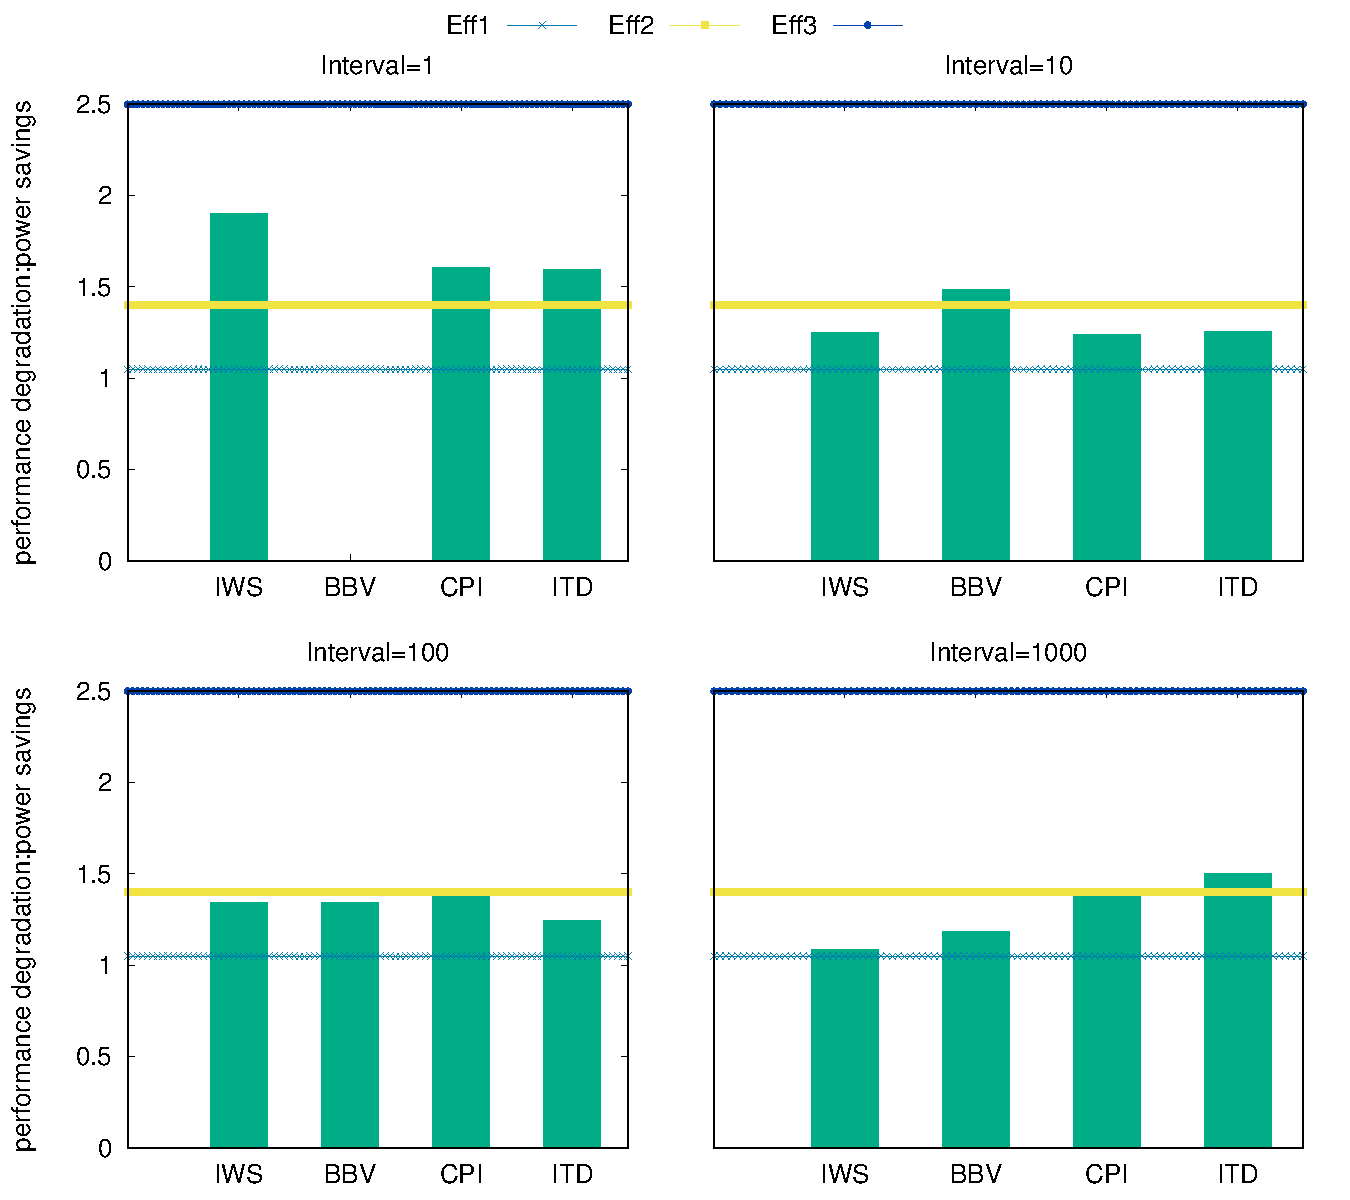
\includegraphics[width=0.99\columnwidth]{figs/ratiodvfs}
  \end{center}
  \caption{Shorter interval sizes result in much more aggressive voltage and frequency settings overall.} 

  \label{fig:ratiodvfs}
\end{figure}

